\documentclass[aspectratio=169,notes]{beamer}
% \documentclass[aspectratio=169]{beamer}
\usetheme[faculty=phil]{fibeamer}
\usepackage{polyglossia}
\setmainlanguage{english} %% main locale instead of `english`, you
%% can typeset the presentation in either Czech or Slovak,
%% respectively.
\setotherlanguages{russian} %% The additional keys allow
%%
%%   \begin{otherlanguage}{czech}   ... \end{otherlanguage}
%%   \begin{otherlanguage}{slovak}  ... \end{otherlanguage}
%%
%% These macros specify information about the presentation
\title[AGLA1]{Analytical Geometry and Linear Algebra I, Lab 4} %% that will be typeset on the
\subtitle{Inverse Matrix \\ Change of basis \\ \   
         } %% title page.
\author{Oleg Bulichev}
%% These additional packages are used within the document:
\usepackage{ragged2e}  % `\justifying` text
\usepackage{booktabs}  % Tables
\usepackage{tabularx}
\usepackage{tikz}      % Diagrams
\usetikzlibrary{calc, shapes, backgrounds}
\usepackage{amsmath, amssymb}
\usepackage{url}       % `\url`s
\usepackage{listings}  % Code listings
% \usepackage{subfigure}
\usepackage{floatrow}
\usepackage{subcaption}
\usepackage{mathtools}
\usepackage{todonotes}
\usepackage{fontspec}
\usepackage{multicol}
\usepackage{pdfpages}
\usepackage{wrapfig}
\usepackage{animate}
\usepackage{booktabs}
\usepackage{multirow}

\graphicspath{{resources/}}
\frenchspacing

\setbeamertemplate{caption}[numbered]
\usetikzlibrary{graphs}

% \usepackage[backend=biber,style=ieee,autocite=footnote]{biblatex}
% \addbibresource{biblio.bib}
% \DefineBibliographyStrings{english}{%
%   bibliography = {References},}

\newcommand{\oleg}[2][] {\todo[color=red, #1] {OLEG:\\ #2}}
\newcommand{\fbckg}[1]{\usebackgroundtemplate{\includegraphics[width=\paperwidth]{#1}}}%frame background

\usepackage[framemethod=TikZ]{mdframed}
\newcommand{\dbox}[1]{
\begin{mdframed}[roundcorner=3pt, backgroundcolor=yellow, linewidth=0]
\vspace{1mm}
{#1}
\vspace{1mm}
\end{mdframed}
}

\begin{document}
\setlength{\abovedisplayskip}{0pt}
\setlength{\belowdisplayskip}{0pt}
\setlength{\abovedisplayshortskip}{0pt}
\setlength{\belowdisplayshortskip}{0pt}

\fbckg{fibeamer/figs/title_page.png}
\frame[c]{\setcounter{framenumber}{0}
    \usebeamerfont{title}%
    \usebeamercolor[fg]{title}%
    \begin{minipage}[b][6.5\baselineskip][b]{\textwidth}%
        \textcolor{black}{\raggedright\inserttitle}
    \end{minipage}
    % \vskip-1.5\baselineskip

    \usebeamerfont{subtitle}%
    \usebeamercolor[fg]{framesubtitle}%
    \begin{minipage}[b][3\baselineskip][b]{\textwidth}
        \raggedright%
        \insertsubtitle%
    \end{minipage}
    \vskip.25\baselineskip
}
%   \frame[c]{\maketitle}
\note{
    \begin{enumerate}
        \item Смену базиса давать через вывод формулы: вектор - фреймлесс, а координаты вектора - нет. Поэтому можно вот выразить ручку по разному. Все на основе линейных комбинаций. \smallskip

        Есть 2 твои формулы - бро $E' = EA$ и $Ex=E'x'$. Разновидность бро $Ex = Eb + E'x'$, где $E = [e_1\ e_2\ e_3]$, $E = [e'_1\ e'_2\ e'_3]$ 

        \item Забить на слайды и объяснять на маркерах, ручках и доске про смену базиса

    \end{enumerate}
}

\fbckg{fibeamer/figs/common.png}


\begin{frame}[c]{Questions from the class}
\framesubtitle{}
\centering
    \textit{ \Large No questions for today}
\end{frame}

\begin{frame}[t]{Inverse Matrix}
\framesubtitle{Why do we need it?}
\vspace{-3ex}
    \begin{figure}[H]
        \centering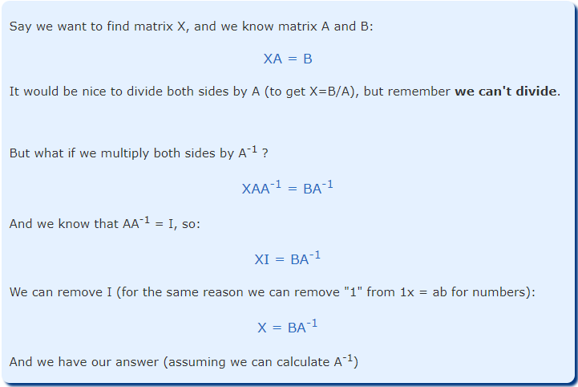
\includegraphics[height=6cm,width=1\textwidth,keepaspectratio]{inverse_why.png}
        % \caption{caption_name}
        \label{fig:inverse_why.png}
    \end{figure}
\end{frame}

\begin{frame}[t]{Inverse Matrix}
\framesubtitle{Properties}
    \begin{enumerate}
        \item $det(A^{-1}) = \dfrac{1}{det(A)}$
        \item $(AB)^{-1}=A^{-1}B^{-1}$
        \item $(A^{-1})^T=(A^T)^{-1}$
        \item $(kA)^{-1}=\dfrac{A^{-1}}{k}$
        \item $(A^{-1})^{-1}=A$
    \end{enumerate}
\end{frame}

\begin{frame}[t]{Inverse Matrix}
\framesubtitle{How to find}
    There are 2 ways:
    \begin{enumerate}
        \item Classical approach
        \item Gauss-Jordan
    \end{enumerate}
\end{frame}

\begin{frame}[t]{Inverse Matrix: Classical Approach}
\framesubtitle{Theory}
   $\underset{2 \times 2}{A}^{-1} = \dfrac{C^T}{det(A)}$, where $C$ is a matrix of \textit{cofactors}. \smallskip
   
   $\underset{2 \times 2}{C} = \begin{bmatrix} C_{11} & C_{12} \\ C_{21} & C_{22} \end{bmatrix}$, where $C_{ij} = (-1)^{i+j}M_{ij}$ --- (we met it on previous lab (lab 3))
\end{frame}

\begin{frame}[t]{Inverse Matrix: Classical Approach}
\framesubtitle{Case Study}
\vspace{-0.5cm}
    \begin{multicols}{2}
        $A=\begin{bmatrix}
        1 & 2\\ 
        3 & 4 
        \end{bmatrix}$. Let's find $A^{-1}$.
        \begin{enumerate}
            \item Find a determinant (shouldn't be equal to $0$, otherwise $\rightarrow$ stop calculations).

            $det(A)=1 \cdot 4 - 2 \cdot 3 = -2$
            \item Find Cofactor matrix
            $C_{11} = (-1)^{1+1}M_{11}=(-1)^2|4|=4$\\
            $C_{12} = (-1)^{1+2}M_{12}=(-1)^3|3|=-3$\\
            $C_{21} = (-1)^{2+1}M_{21}=(-1)^3|2|=-2$\\
            $C_{22} = (-1)^{2+2}M_{22}=(-1)^4|1|=1$\\
            $C = \begin{bmatrix} 4 & -3\\ -2 & 1\end{bmatrix}$
            \item Transpose cofactor matrix\\
            $C^T=\begin{bmatrix} 4 & -2\\ -3 & 1\end{bmatrix}$
            \item Substitute it to the main formula \medskip

            $A^{-1}=\dfrac{\begin{bmatrix} 4 & -2\\ -3 & 1\end{bmatrix}}{-2} = \begin{bmatrix} -2 & 1\\ 1.5 & -0.5\end{bmatrix}$
        \end{enumerate}
    \end{multicols}
\end{frame}

\begin{frame}[t]{Inverse Matrix: Gauss-Jordan}
\framesubtitle{Core Idea \& Case study ($2 \times 2$)}
    The 
\end{frame}

\note{Не забудь, нужно подумать как оформить эту штуку честь по чести. А то вроде ее и понимают, но времени не много. Как это оформить нормально.}

\begin{frame}[t]{Reference material}
    % \framesubtitle{OnlineMschool}
    \Large
    \begin{itemize}
        \item \href{https://onlinemschool.com/math/library/matrix/inverse/}{Inverse Matrix (OnlineMschool)}
        \item \href{https://en.wikipedia.org/wiki/Gaussian_elimination}{Gauss-Jordan (Wiki)}
        \item \href{https://onlinemschool.com/math/library/matrix/rank/}{Matrix Rank (OnlineMschool)}
    \end{itemize}
\end{frame}

\fbckg{fibeamer/figs/last_page.png}
\frame[plain]{}

\end{document}